\documentclass[12pt]{article}
\usepackage{graphicx}
\usepackage{hyperref}
\usepackage{cite}
\usepackage{float} % for [H] anchoring method
\usepackage[top=1.4in, bottom=1.4in, left=1.4in, right=1.4in]{geometry}
\graphicspath{ {pngs/} }
\usepackage{mdframed}

\newcommand{\specialcell}[2][c]{%
	\begin{tabular}[#1]{@{}c@{}}#2\end{tabular}}

\begin{document}
\title{CSE326 Semester Project Design Spec: Anttris}
\author{Team \#5\\\\Chris Aikman\\Benji Cope\\Skyler Manzanares\\Hugo Rivera\\Sean Turner}
\maketitle

\section{Project Overview}
% I will work on all of this section (Section 1) CA
\subsection{Scope and Objectives}
% CA
% HR
\subsection{Supplementary Requirements}
% CA
\section{Customer Requirements}
% SM
\subsection{Use-Case Diagrams}
    \begin{figure}[H]
        \centering
        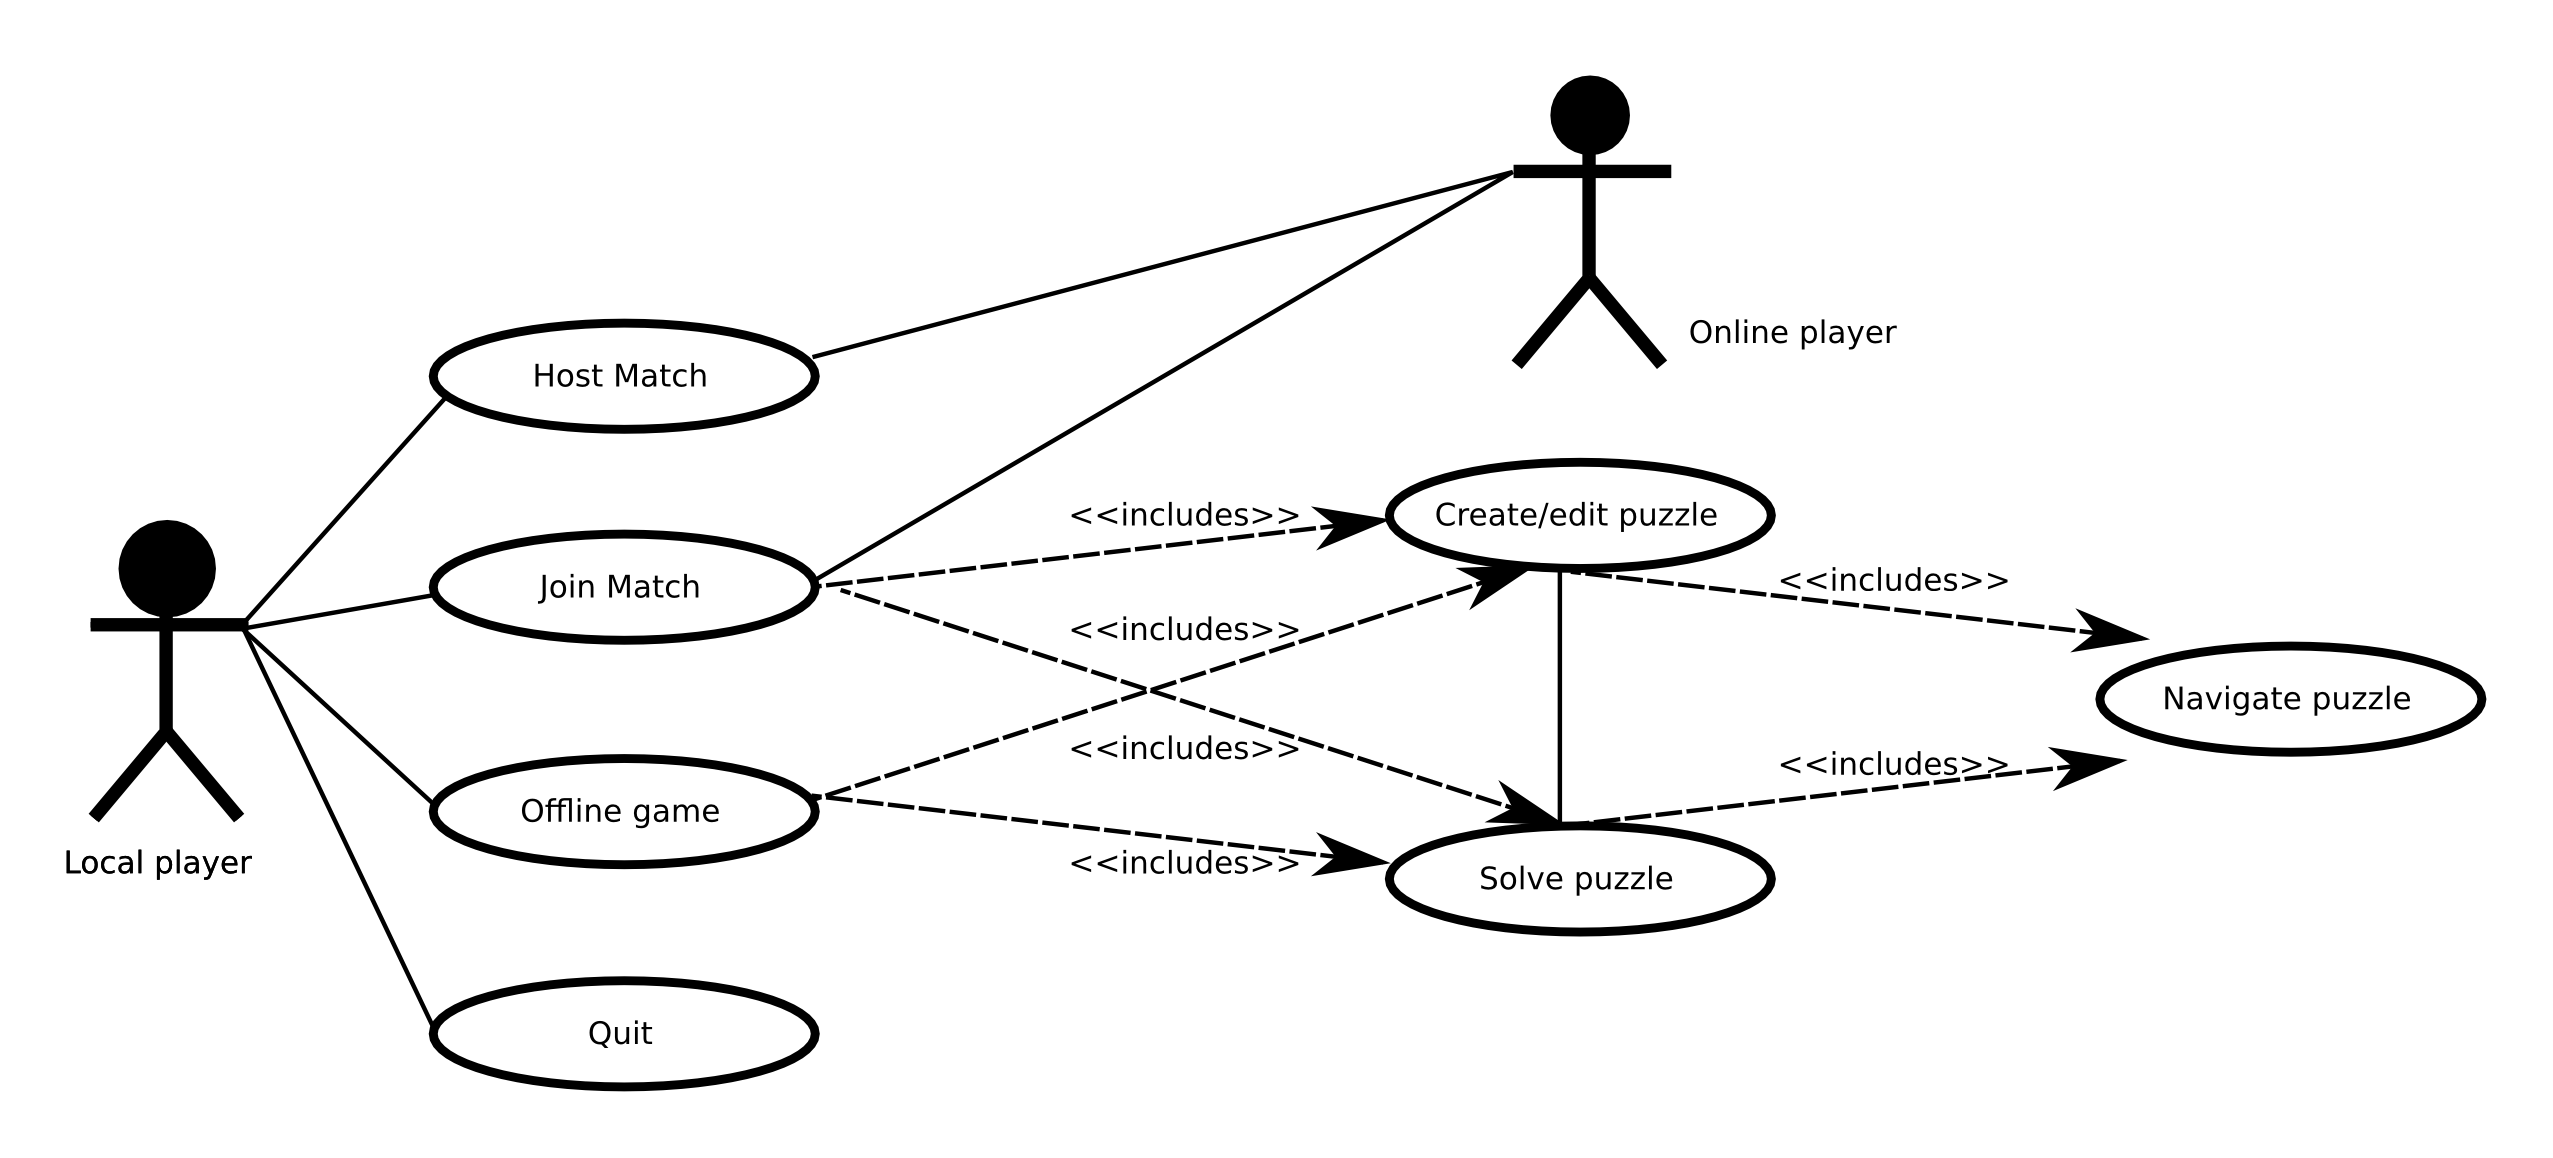
\includegraphics[width=6in]{use_cases.png}
        \caption{Use Case Diagram}
    \end{figure}

\subsection{Actor Descriptions}
    \begin{description}
        \item[Local player] is the local user and has full
            access to the mouse and keyboard or touchscreen interface.
        \item[Online player] is a non-local player. There is two-way
            communication between this type of player and the local player.
            There may be 0 or more online players.
        \item[The Host] has special powers, may disconnect other players and
            block players from selecting different puzzles. This player could
            be Local or Online.
    \end{description}

\subsection{Use-case Descriptions}
\begin{mdframed}
    \subsubsection{Host match}
    \begin{description}
        \item[Entry conditions] Internet connection.
        \item[Exit conditions] Will return to game menu. All players
            disconnected or all puzzles have been solved.
        \item[Participating Actors] Online player and local player.
        \item[Flow of events]:
            \begin{enumerate}
                \item The user presses the appropriate menu button.
                \item User creates a game, selects number of players and game
                    type
                \item User shares (friendly looking) match ID with other
                    players. These players may connect to the match
                \item Puzzle Selector appears.
                \item The user may configure the game with this screen.
                    This
                    entails choosing a puzzle and a game mode (edit or solve).
                    Other players can be prevented from making such
                    modifications.
                \item This Puzzle Selector will create a Puzzle Scene
                \item The scene will change from the main menu to the Puzzle
                    Scene.
                \item Additional view-ports will be added to the game screen. 
                These show the progress of online players in an interface
                similar to the local player's puzzle.

            \end{enumerate}
    \end{description}
\end{mdframed}

\begin{mdframed}
    \subsubsection{Join match}
    \begin{description}
        \item[Entry conditions] Internet connection. The menu must be present.
        \item[Exit conditions] Will return to game menu. All players
            disconnected or all puzzled have been solved.
        \item[Participating Actors] Online player and local player.
        \item[Flow of events]:
            \begin{enumerate}
                \item The user presses the appropriate menu button.
                \item Puzzle Selector appears.
                \item The user may configure the game with this screen, if
                    the game host allows it. This would
                    entail choosing a puzzle and a game mode (edit or solve).
                \item This Puzzle Selector will create a Puzzle Scene
                \item The scene will change from the main menu to the Puzzle
                    Scene.
                \item Additional view-ports will be added to the game screen. 
                These show the progress of online players in an interface
                similar to the local player's puzzle.
            \end{enumerate}
    \end{description}
\end{mdframed}


\begin{mdframed}
    \subsubsection{Offline game}
    \begin{description}
        \item[Entry conditions] Menu must be present.
        \item[Exit conditions] Will return to game menu. Puzzle has been
            solved.
        \item[Participating Actors] Local player.
        \item[Flow of events]:
            \begin{enumerate}
                \item User selects the appropriate menu button.
                \item Puzzle Selector appears.
                \item The user may configure the game with this screen. This
                    entails choosing a puzzle and a game mode (edit or solve).
                \item This Puzzle Selector will create a Puzzle Scene
                \item The scene will change from the main menu to the Puzzle
                    Scene.
            \end{enumerate}
    \end{description}
\end{mdframed}


\begin{mdframed}
    This use case includes the Host Match, Join Match and Offline Game
    use cases.
    \subsubsection{Edit puzzle}
    \begin{description}
        \item[Entry conditions] A Puzzle Scene must be loaded and edit mode
            must be activated.
        \item[Exit conditions] Will return to game menu. The puzzle may be
            saved to the disk.
        \item[Participating Actors] Online player or local player.
        \item[Flow of events]:
            \begin{enumerate}
                \item The user navigates the puzzle
                \item If a position on the grid is selected, the Block Modifier
                    is presented. This position may be empty or it may
                    contain a block.
                \item The user may change properties of the block using this
                    screen.
                \item Blocks may be added or removed using this same screen.
            \end{enumerate}
            Puzzle preview:
            \begin{enumerate}
                \item User may press the preview button
                \item The user will try the puzzle in Solve Puzzle mode until
                    that mode's exit conditions are met.
                    A special banner will graphically indicate preview mode.
                \item The solving scene will have a special button for
                    returning to the editing scene
            \end{enumerate}
    \end{description}
\end{mdframed}


\begin{mdframed}
    This use case includes the Host Match, Join Match and Offline Game
    use cases.
    \subsubsection{Solve puzzle}
    \begin{description}
        \item[Entry conditions] A Puzzle Scene must be loaded and solve mode
            must be activated.
        \item[Exit conditions] Will return to game menu or puzzle editor.
            If the game is over, an overview of results will be shown and the
            steps taken to solve the puzzle may be saved to the disk.
        \item[Participating Actors] Online player or local player.
        \item[Flow of events]:
            \begin{enumerate}
                \item The user navigates the puzzle
                \item If a block is selected, the block runs any associated
                    Block Action.
                \item These Block Actions may modify the block's properties or
                    request the addition or removal of blocks, including the
                    selected block, from the Grid Manager.
                \item This sequence is repeated until the winning block is
                    found, the user quits, or a losing condition is met.
                \item User's actions may be mirrored on an online player's
                    screen, likewise, separate Puzzle Scenes  may be updated
                    with any moves made by other players.
            \end{enumerate}
    \end{description}
\end{mdframed}


\begin{mdframed}
    \subsubsection{Navigate puzzle}
    This use case includes the Solve puzzle and Edit puzzle use cases.
    \begin{description}
        \item[Entry conditions] Puzzle scene loaded and permission to move.
            Input devices must be functional.
        \item[Exit conditions] The game must offer continuous feedback.
            If the entry conditions are met, any further input must be
            acted on as soon as possible.
        \item[Participating Actors] Online player and local player.
        \item[Flow of events]:
        	\\
            Camera motion:
            \begin{enumerate}
                \item User drags with a mouse or touchscreen
                \item The camera changes position
            \end{enumerate}

            Block selection:
            \begin{enumerate}
                \item User clicks with mouse or taps on touchscreen
                \item The 3D coordinates are translated into a position on
                    a game ``board.''
                \item The Grid Manager is notified of input and the grid
                    position.
                \item If a block is present there, it is selected and activated.
                    Exact actions depend on the game mode.
                \item If a block is not present, the space is selected. This
                    is only useful in edit mode.
                \item The user may end the game at any point through the pause
                    menu.
            \end{enumerate}

    \end{description}
\end{mdframed}


\begin{mdframed}
    \subsubsection{Quit}
    \begin{description}
        \item[Entry conditions] Game must be running. This action is
            asynchronous and may activate at any point.
        \item[Exit conditions] Game, be gone!
        \item[Participating Actors] Local player.
        \item[Flow of events]:
            \begin{enumerate}
                \item User presses the quit button on a menu
                \item or User presses appropriate sequence of keys, such as
                    the escape key or the alt and F4 combo.
                \item Some data may be saved, such as the puzzle being currently 
                edited.
                \item The program shuts down gracefully.
            \end{enumerate}
    \end{description}
\end{mdframed}



\section{Architectural Design}
% HR
\subsection{Subsystem Architecture}
% SM
\begin{figure}[H]
    \centering
    
\includegraphics[width=6in]{subsys_arch.png}
    \caption{Use Case Diagram}
\end{figure}
The two primary subsystems of Anttris are the puzzle-solving system and the online system.

The puzzle-solving system is composed generically over a puzzle viewer and attached event
handling that allows interaction with the puzzle. Both offline games and online ones use 
the puzzle viewer, as does the unique puzzle-editing mode. The puzzle viewer is used by
all three unique modes, and works with our 3D model interaction system to provide
interactivity. This system is built on the Godot 3d Engine, which uses OpenGL.

The online system breaks down immediately into host mode or remote client mode. The host 
mode interfaces with the application-generic session-host system, which works in conjunction
with the session lobby to facilitate remote clients to connect and play against the host. 
Remote clients also work closely with the session lobby to find hosts to play against. Both
the session lobby and the session-host system work with the Godot Online Subsystem to provide
connectivity. The Godot Online Subsystem is built over tcp-udp/ip.

\subsection{Deployment Model}
% HR
\section{Use Case Realization Design}
% HR, I did Use Cases last time, I can work on all of this
\section{Subsystem Design}
% I will work on all of this section (Section 5) CA
\subsection{Subsystem A}
% CA
\subsection{Subsystem B}
% CA
\section{Human Interfaces}
% SM, I will work on all of this section (Section 6), I already have most of the UI design done already CA
\section{System/Data Dependencies \& Requirements}
% ST, BC
\section{Testing Plan}
% ST, BC
\section{Appendices}
% ST
\subsection{Project Status}
% ST

\bibliographystyle{acm}
\bibliography{team5-design-spec}
\end{document}
